% -*- root: ../main.tex -*-
% Chapter Template
\tikzset{declare function={
    rise(\t,\ta,\n) = and(\t >= 0, \t < \ta/(2^(2/\n))) * 2*(\t/\ta)^\n    +
    and(\t >= \ta/2^(2/\n), \t< \ta) * ((-2)*(\t/\ta)^\n + 4*(\t/\ta)^(\n/2) - 1)     +
     (\t>\ta) * (1);
  },
  declare function={
    fall(\t,\tb) = exp(-\t/\tb);
  },
  declare function={
    teres(\t,\ta,\tb,\n,\I,\e) = (\I/\e)*fall(\t,\tb)*rise(\t,\ta,\n);
  }}

\chapter{The Terespolsky Function} % Main chapter title

\label{ChapterTeres} % Change X to a consecutive number; for referencing this chapter elsewhere, use \ref{ChapterX}

\lhead{\chaptername~\thechapter. \emph{The Terespolsky Function}} % Change X to a consecutive number; this is for the header on each page - perhaps a shortened title
\begin{quote}
\note[BRT]{Chapter abstract goes here!}
\end{quote}

\section{Overview}


\section{Function Definition and Properties}
The Terespolsky function is an approximation of the Heidler function with the advantage that it has an analytical solution in the frequency domain. Moreover it is still ``customizable'', meaning that the steepness of the graph, the rise and fall times and peak current can all be modified. This allows for analyses using 10/350, 8/20 and any other lightning waveforms required.

The Terespolsky function is defined in \eqnref{eqn:TF}
\begin{equation}
i(t) = \frac{I_0}{\eta} e^{-\frac{t}{\tau_2}} \left\{
  \begin{array}{l l}
    2 \left( \frac{t}{\tau_1} \right )^n & \quad \textrm{for $0 \leq t < \frac{\tau_1}{2^{\frac{2}{n}}}$} \\
    -2 \left( \frac{t}{\tau_1} \right )^n +4 \left( \frac{t}{\tau_1} \right )^{\frac{n}{2}} -1 & \quad \textrm{for $\frac{\tau_1}{2^{\frac{2}{n}}} \leq t < \tau_1$} \\
    1 & \quad \textrm{for $t \geq \tau_1$}
  \end{array} \right.
\label{eqn:TF}
\end{equation}
Where: \\
\begin{tabular}{cll}
	$I_0$ & = & Peak current [kA] \\
	$\eta$ & = & Correction factor of peak current \\
	$\tau_1$ & = & Rise time constant [s] \\
	$\tau_2$ & = & Fall time constant [s] \\
	$n$ & = & Steepness factor
\end{tabular}\\

Modifying these properties gives the desired lightning current waveform. An example plot of this function can be seen in \figref{fig:TeresFuncEX}.
\begin{figure}[]
	\centering
	\tikzsetnextfilename{TeresFuncEx}
	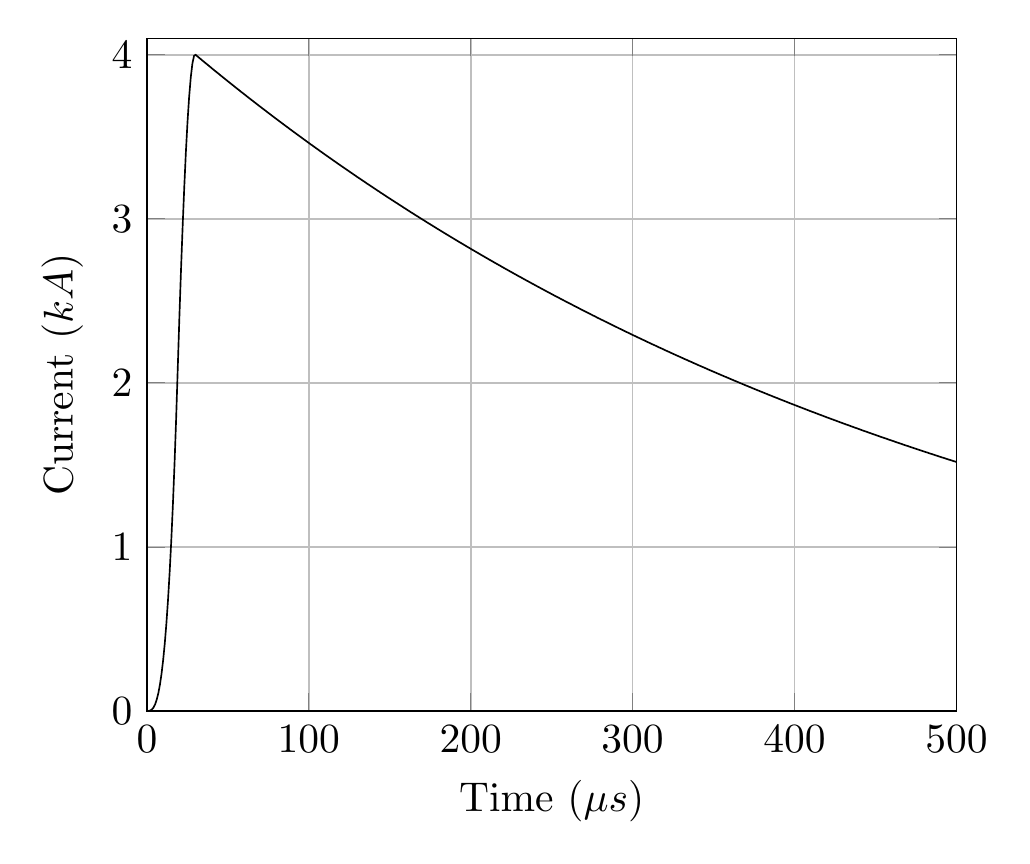
\begin{tikzpicture}[
  scale = 1.5,
]
  \begin{axis}[
    xlabel=Time ($\mu s$),
    ylabel=Current ($kA$),
    grid=both,
    /pgf/number format/1000 sep={},
    xmin=0,
    xmax=500e-6,
    ymin=0,
    ymax=4.1,
    cycle list name=linestyles*,
    scaled x ticks={base 10:6},
    xtick scale label code/.code={},
    samples=500
  ]
    
    \addplot+[domain=0:500e-6] {teres(\x, 30e-6, 485e-6, 3, 4, 0.94)};

  \end{axis}
\end{tikzpicture}
	\caption{Graph of an example Terespolsky function lightning current waveform.}
	\label{fig:TeresFuncEX}
\end{figure}
As with the Heidler function, the Terespolsky function can be rewritten as in \eqnref{eqn:TFSmall}.
\begin{equation}
i(t) = \frac{I_0}{\eta} x \left( t \right) y \left( t \right)
\label{eqn:TFSmall}
\end{equation}
where the function in \eqnref{eqn:TFrise}
\begin{equation}
	x \left( t \right) = \left\{
	  \begin{array}{l l}
	    2 \left( \frac{t}{\tau_1} \right )^n & \quad \textrm{for $0 \leq t < \frac{\tau_1}{2^{\frac{2}{n}}}$} \\
	    -2 \left( \frac{t}{\tau_1} \right )^n +4 \left( \frac{t}{\tau_1} \right )^{\frac{n}{2}} -1 & \quad \textrm{for $\frac{\tau_1}{2^{\frac{2}{n}}} \leq t < \tau_1$} \\
	    1 & \quad \textrm{for $t \geq \tau_1$}
	  \end{array} \right.
	\label{eqn:TFrise}
\end{equation}
is the current-rise function and the function in \eqnref{eqn:TFfall}
\begin{equation}
	y \left( t \right) = e^{-\frac{t}{\tau_2}}
	\label{eqn:TFfall}
\end{equation}
is the current-decay function.

It is clear that the Terespolsky function takes the same form as the Heidler function (see \secref{sec:bg_heidler}). The difference is in $x \left( t \right)$ which is not directly integrate-able in the Heidler function but can be integrated and hence transformed into the frequency domain in the Terespolsky function.

\subsection{Steepness Factor}


\subsection{Rise Time}


\subsection{Fall Time}


\subsection{Delayed Function}


\section{Time Domain Analysis}


\section{Frequency Domain Analysis}


\section{Conslusion}